% 本模板根据中国科学院大学本科生公共必修课程《基础物理实验》Word模板格式编写
% 本模板由Shing-Ho Lin和Jun-Xiong Ji于2022年9月共同完成, 旨在方便LaTeX原教旨主义者和被Word迫害者写实验报告, 避免Word文档因插入过多图与公式造成卡顿. 
% 如有任何问题, 请联系: linchenghao21@mails.ucas.ac.cn
% This is the LaTeX template for experiment report of Experimental Physics courses, based on its provided Word template. 
% This template is completed by the joint collabration of Shing-Ho Lin and Junxiong Ji in September 2022. 
% Adding numerous pictures and equations leads to unsatisfying experience in Word. Therefore LaTeX is better. 
% Feel free to contact us via: linchenghao21@mails.ucas.ac.cn

\documentclass[11pt]{article}

\usepackage[a4paper]{geometry}
\geometry{left=2.0cm,right=2.0cm,top=2.2cm,bottom=2.2cm}

\usepackage{ctex} % 支持中文的LaTeX宏包
\usepackage{amsmath,amsfonts,graphicx,subfigure,amssymb,bm,amsthm,mathrsfs,mathtools,breqn} % 数学公式和符号的宏包集合
\usepackage{algorithm,algorithmicx} % 算法和伪代码的宏包
\usepackage[noend]{algpseudocode} % 算法和伪代码的宏包
\usepackage{fancyhdr} % 自定义页眉页脚的宏包
\usepackage[framemethod=TikZ]{mdframed} % 创建带边框的框架的宏包
\usepackage{fontspec} % 字体设置的宏包
\usepackage{adjustbox} % 调整盒子大小的宏包
\usepackage{fontsize} % 设置字体大小的宏包
\usepackage{tikz,xcolor} % 绘制图形和使用颜色的宏包
\usepackage{multicol} % 多栏排版的宏包
\usepackage{multirow} % 表格中合并单元格的宏包
\usepackage{pdfpages} % 插入PDF文件的宏包
\RequirePackage{listings} % 在文档中插入源代码的宏包
\RequirePackage{xcolor} % 定义和使用颜色的宏包
\usepackage{wrapfig} % 文字绕排图片的宏包
\usepackage{bigstrut,multirow,rotating} % 支持在表格中使用特殊命令的宏包
\usepackage{booktabs} % 创建美观的表格的宏包
\usepackage{circuitikz} % 绘制电路图的宏包
\usepackage[inline]{enumitem}
\usepackage{tabularx}

\usepackage{indentfirst}
\setlength{\parindent}{2em}
\setlength{\abovecaptionskip}{2pt}
\setlength{\belowcaptionskip}{2pt}
\setlength{\intextsep}{6pt}
\setlength{\floatsep}{6pt}

\definecolor{dkgreen}{rgb}{0,0.6,0}
\definecolor{gray}{rgb}{0.5,0.5,0.5}
\definecolor{mauve}{rgb}{0.58,0,0.82}
\lstset{
  frame=tb,
  aboveskip=1mm,
  belowskip=1mm,
  showstringspaces=false,
  columns=flexible,
  framerule=1pt,
  rulecolor=\color{gray!35},
  backgroundcolor=\color{gray!5},
  basicstyle={\small\ttfamily},
  numbers=none,
  numberstyle=\tiny\color{gray},
  keywordstyle=\color{blue},
  commentstyle=\color{dkgreen},
  stringstyle=\color{mauve},
  breaklines=true,
  breakatwhitespace=true,
  tabsize=3,
}

% 轻松引用, 可以用\cref{}指令直接引用, 自动加前缀. 
% 例: 图片label为fig:1
% \cref{fig:1} => Figure.1
% \ref{fig:1}  => 1
\usepackage[capitalize]{cleveref}
% \crefname{section}{Sec.}{Secs.}
\Crefname{section}{Section}{Sections}
\Crefname{table}{Table}{Tables}
\crefname{table}{Table.}{Tabs.}

\setmainfont{Palatino Linotype.ttf}
\setCJKmainfont{SimHei.ttf}
% \setCJKsansfont{Songti.ttf}
% \setCJKmonofont{SimSun.ttf}
\punctstyle{kaiming}
% 偏好的几个字体, 可以根据需要自行加入字体ttf文件并调用

\renewcommand{\emph}[1]{\begin{kaishu}#1\end{kaishu}}

%改这里可以修改实验报告表头的信息
\newcommand{\experiName}{测量金属的杨氏模量}
\newcommand{\supervisor}{石琛}
\newcommand{\name}{张欣培}
\newcommand{\studentNum}{2022K8009922001}
\newcommand{\class}{01}
\newcommand{\group}{10}
\newcommand{\seat}{}
\newcommand{\dateYear}{2023}
\newcommand{\dateMonth}{12}
\newcommand{\dateDay}{4}
\newcommand{\room}{教710}
\newcommand{\others}{$\square$}
\newcommand{\othersYes}{$\square$\hspace{-1em}$\surd$}
%% 如果是调课、补课, 改为: $\square$\hspace{-1em}$\surd$
%% 否则, 请用: $\square$
%%%%%%%%%%%%%%%%%%%%%%%%%%%

\begin{document}

%若需在页眉部分加入内容, 可以在这里输入
% \pagestyle{fancy}
% \lhead{\kaishu 测试}
% \chead{}
% \rhead{}

\begin{center}
    \LARGE \bf 《\, 基\, 础\, 物\, 理\, 实\, 验\, 》\, 实\, 验\, 报\, 告
\end{center}

\begin{center}
    \noindent \emph{实验名称}\underline{\makebox[25em][c]{\experiName}}
    \emph{指导教师}\underline{\makebox[8em][c]{\supervisor}}\\
    \emph{姓名}\underline{\makebox[6em][c]{\name}} 
    % 如果名字比较长, 可以修改box的长度"6em"
    \emph{学号}\underline{\makebox[10em][c]{\studentNum}}
    \emph{分班分组及座号} \underline{\makebox[5em][c]{\class \ -\ \group \ -\ \seat }\emph{号}} (\emph{例}:\, 1\,-\,04\,-\,5\emph{号})\\
    \emph{实验日期} \underline{\makebox[3em][c]{\dateYear}}\emph{年}
    \underline{\makebox[2em][c]{\dateMonth}}\emph{月}
    \underline{\makebox[2em][c]{\dateDay}}\emph{日}
    \emph{实验地点}\underline{{\makebox[4em][c]\room}}
    \emph{调课/补课} \underline{\makebox[3em][c]{\others\ 是}}
    \emph{成绩评定} \underline{\hspace{5em}}
    {\noindent}
    \rule[8pt]{17cm}{0.2em}
\end{center}

\begin{center}
    \Large \bf 第一部分\qquad 实验内容
\end{center}

\section{实验目的}

\begin{enumerate}
    \item 熟练使用不同的长度测量工具,了解其测量范围和优缺点;
    \item 理解各种静态方法测杨氏模量及其测量微小位移方法的原理及优缺点,了解动态法测杨氏模量的原理;
    \item 熟悉霍尔位置传感器的特性,完成样品的测量和对霍尔位置传感器定标,理解传感器特定曲线对测量的意义;
    \item 了解光杠杆法的放大原理和适用条件;
    \item 学会读数望远镜、读数显微镜的调节;
    \item 学习用逐差法、作图法和最小二乘法处理数据;
    \item 学会计算各物理量的不确定度,并用不确定度正确表达实验结果。
\end{enumerate}

\section{实验器材}
    CCD杨氏弹性模量测量仪(LB-YM1型)、杭州大华DHY-A霍尔位置传感器法杨氏模量测定仪(底座固定箱、读数显微镜及调节机构、
    SS495A 型集成霍尔位置传感器、 测试仪、 磁体、支架、加力机构等)、DHY-2A 型动态杨氏模量测试台、
    样品(黄铜、铸铁)(长条、圆条)、样品(钼丝)螺旋测微器、游标卡尺、钢直尺、钢卷尺。
\section{实验原理}
\begin{enumerate}
    \item 杨氏模量
    \par \hspace*{2em}	
    由胡克定律,$\frac{F}{S}=Y\frac{\Delta L}{L}$,其中F为力,S为截面积,L为物体总长度,L为物体伸长量,$\frac{F}{S}$称为正应力,$\frac{\Delta L}{L}$称为线应力。代入$S=\frac{\pi d^2}{4}$得$Y=\frac{4FL}{\pi d^2\Delta L}$。Y称为杨氏弹性模量,国际单位制下单位是$N/m^2$。杨氏模量可类比弹簧的劲度系数,但金属的伸长和弹簧的伸长不同。本实验中,若金属丝样品有弯曲,局部类弹簧,会对测量产生影响。
    \item 微小长度测量方法
    \par \hspace*{2em}直接测量:在实际测量中,由于金属丝伸长量$\Delta L$的值很小,约${10}^{-1}mm$数量级。因此这里的测量采用显微镜和CCD 成像系统进行测量。CCD摄像机的镜头将显微镜的光学图像汇聚到CCD(Charge Coupled Device,电荷耦合器件)上,再变成视频电信号,经视频电缆传送到显示器,即可供多人同时观测。
    \par \hspace*{2em}间接测量:将长度转化为其他对距离敏感的物理量,如电/磁,运动周期等,或将长度变化通过光学方式放大一定倍数。
    \item 拉伸法
    \par \hspace*{2em}直接对样品进行拉伸,测量样品原长度、样品直径、样品受力、样品长度变化。由于样品长度变化很小,认为样品直径未变化。经过数据处理后,根据$Y=\frac{4FL}{\pi d^2\Delta L}$计算杨氏模量。
    \item 霍尔法
    \par \hspace*{2em} 霍尔元件置于磁感强度为B的磁场中,在垂直于磁场方向通以电流I,则与这二者垂直的方向上将产生霍尔电势差$U_H=K\cdot I\cdot B$。K为霍尔灵敏度。
    \par \hspace*{2em} 如果保持霍尔元件的电流不变,而使其在一个均匀梯度的磁场中移动时,则输出的霍尔电势差变化量为:${\Delta U}_H=K\cdot I\cdot\frac{dB}{dZ}\cdot\Delta Z$。$\Delta Z$为位移量。于是,当位移较小时(<2mm),可以通过测量霍尔传感器电压变化计算位移量。
    \par \hspace*{2em}为实现均匀梯度的磁场,可以如图\ref{fig:1}所示两块相同的磁铁(磁铁截面积及表面感应强度相同)相对位置,即N 极与N 极相对,两磁铁之间留一等间距间隙,霍尔元件平行于磁铁放在该间隙的中轴上。间隙大小要根据测量范围和测量灵敏度要求而定,间隙越小,磁场梯度就越大,灵敏度就越高。磁铁截面要远大于霍尔元件,以尽可能的减小边缘效应的影响,提高测量精确度。
    \par \hspace*{2em}在横梁弯曲的情况下,杨氏模量$E=\frac{d^3\cdot M g}{4a^3\cdot b\cdot\Delta Z}$。其中:d为两刀口之间的距离;M为所加拉力对应的质量;a为梁的厚度;b为梁的宽度;$\Delta Z$为梁中心由于外力作用而下降的距离;g为重力加速度。
    \begin{figure}[H]
        \centering
        \begin{minipage}[t]{0.49\linewidth}
            \centering
            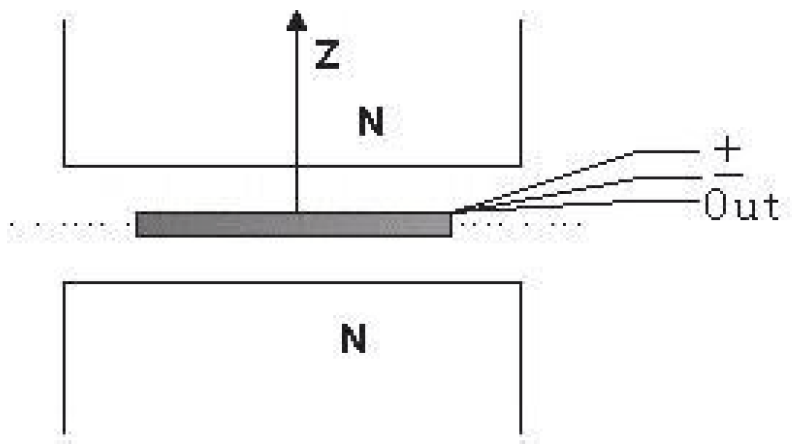
\includegraphics[width=7cm]{Fig/1.png}
            \caption{霍尔法测量示意图}
            \label{fig:1}
        \end{minipage}
        \begin{minipage}[t]{0.49\linewidth}
            \centering
            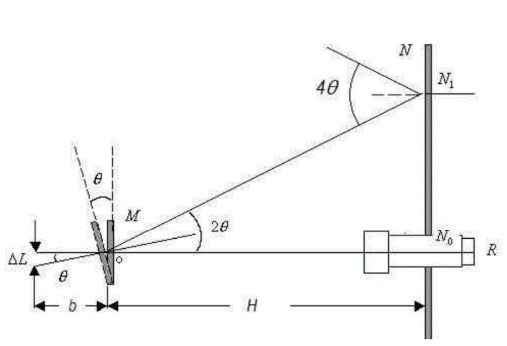
\includegraphics[width=7cm]{Fig/2.png}
            \caption{光杠杆法测量示意图}
            \label{fig:2}
        \end{minipage}
    \end{figure}
    \item 动态法
    \par \hspace*{2em}此方法要测量的是棒的共振频率。通过解微分方程,对于直径d,长为L,质量为m的圆形棒,计算得棒的杨氏弹性模量为$Y=1.6067\frac{L^3mf_1^2}{d^4}$。
    \par \hspace*{2em}测试棒在作基频振动时存在两个节点,它们的位置距离端面0.224L(距离另一端面为0.776L)处,理论上,悬挂点应取在节点处测试棒难于被激振和拾振,为此可在节点两旁选不同点对称悬挂,用外推法找出节点处的共振频率。
    \par \hspace*{2em}另外,固有频率和共振频率的关系是$f_{\text{固}}=f_{\text{共}}\sqrt{1+\frac{1}{4Q^2}}$,其中Q为测试的机械品质因数。为测试的机械品质因素。对于悬挂法测量,一般Q的最小值约为50,共振频率和固有频率相比只偏低0.005\%,本实验中只能测出测试的共振频率,由于两者相差很小。因此,固有频率可用共振频率代替。
    \item 光杠杆法
    \par \hspace*{2em} 由于伸长量难以直接测量,在实验中使用光杠杆放大变化。如图\ref{fig:2},$\Delta L=b\tan{\theta}\approx b\theta$,其中b为光杠杆常数。设伸长量C,由几何关系$2\theta\approx\tan{2\theta}=\frac{C}{2H}$,$\theta=\frac{C}{4H}$, $\Delta L=\frac{bC}{4H}$,得杨氏模量$Y=\frac{16FLH}{\pi d^2bC}$。 

\end{enumerate}


\section{实验内容}
\subsection{拉伸法测定金属的杨氏模量}
\noindent 实验步骤:
\begin{enumerate}
    \item 实验仪器进行调平,打开CCD,调整显微镜底座,使屏幕上能够良好看到刻度。
    \item 用钢卷尺测待测钼丝长度,记为L。
    \item 用螺旋测微器测待测钼丝的直径,测6次取平均值,记为$\bar{d}$。
    \item 读取CCD显示器上的示数,记录显示器初始示数为$l_0$。在钼丝下加砝码,测量加载时钼丝相对长度,记录显示器示数$l_i$和此时钼丝上的砝码质量$M_i$,重复8次。之后依次卸下钼丝下砝码,测量卸载时钼丝相对长度,记录显示器示数${l}_i^'$和此时钼丝上的砝码质量$M_i$。取$l_i$和${l}_i^'$的平均值$\bar{l}_i$。
    \item 整理数据,计算$l_i M_i$,示数差值$\Delta \bar{l}_i=\bar{l}_{i+4}-\bar{l}_i$。由逐差法,不确定度
    \[\Delta(\Delta l)=\frac{\sum_{i = 1}^{n} \Delta \bar{l}_i }{n^2}\]
    质量和长度平均值的平均值与总和$\bar{M},\sum M,\bar{\bar{l}}, \sum \bar{l}$。
    \item 作图法和最小二乘法处理数据。
\end{enumerate}
\noindent 实验数据:
    \par \hspace*{2em}钼丝长度$L=727mm$\qquad 卷尺仪器误差$e=\pm 2mm$
\begin{table}[H]
    \centering
    \caption{钼丝直径}
    \begin{tabular}{|c|c|c|c|c|c|c|c|}
    \hline
        测量次数 & 1 & 2 & 3 & 4 & 5 & 6 & 平均值$\bar{d}$\\ \hline
        d/mm & 0.298  & 0.297  & 0.296  & 0.294  & 0.296  & 0.300 &0.297 \\ \hline
    \end{tabular}
\end{table}
    \par \hspace*{2em}初始示数$l_0=0.55mm$\qquad 千分尺仪器误差$e=\pm 0.005mm$
\begin{table}[H]
    \centering
    \caption{拉伸法测量数据}
    \begin{tabular}{|c|c|c|c|c|c|c|}
    \hline
        $M/g$ & 加载$l_i/mm$ & 卸载$l_i^'/mm$ & $\bar{l}_i/mm$ & $\bar{l}_i\text{修正}/mm$ & $l_i\cdot M_i/(mm\cdot g)$ & $\Delta \bar{l}_i$ \\ \hline
        0 & 0.55 & 0.60  & 0.58  & 0.00  & 0 & ~   \\ \hline
        250 & 0.20  & 0.25  & 0.22  & 0.36  & 90 & 0.80  \\ \hline
        500 & 0.00  & 0.00  & 0.00  & 0.58  & 290 & 0.75 \\ \hline
        750 & -0.20  & -0.20  & -0.20  & 0.78  & 585 & 0.72  \\ \hline
        1000 & -0.40  & -0.40  & -0.40  & 0.98  & 980 & 0.65 \\ \hline
        1250 & -0.60  & -0.55  & -0.58  & 1.16  & 1450 & ~ \\ \hline
        1500 & -0.75  & -0.75  & -0.75  & 1.33  & 1995 & ~ \\ \hline
        1750 & -0.95  & -0.90  & -0.92  & 1.50  & 2625 & ~  \\ \hline
        2000 & -1.05  & ~ & -1.05  & 1.63  & 3260 & ~  \\ \hline
    \end{tabular}
\end{table}

\begin{table}[H]
    \centering
    \begin{tabular}{|c|c|c|c|c|c|c|}
    \hline
        $\Delta l/mm$  & $\sum M$ & $\bar{M}$  & $\sum \bar{l}$ & $\bar{\bar{l}}$  & $\sum \bar{l}^2$ & $\sum M_i l_i$ \\ \hline
        0.182 & 9000 & 1125 & 8.23 & 1.03 & 10.06 & 11275  \\ \hline
    \end{tabular}
\end{table}

最小二乘法公式:设$y=kx+b$,则有
\begin{equation}
    k=\frac{n\cdot \sum\limits_{i = 1}^{n}x_i y_i - \sum\limits_{i = 1}^{n}x_i  \sum\limits_{i = 1}^{n}y_i  }{n\cdot \sum\limits_{i = 1}^{n}x_i^2-{\left(\sum\limits_{i = 1}^{n}x_i\right)}^2} 
    \qquad b=\bar{y}-k\bar{x}
\end{equation}
\par \hspace*{2em} 本实验中,$M=\frac{\pi d^2 }{4gL}Y\cdot \Delta L=k\Delta L$。其中,$\frac{\pi d^2 }{4gL}=9.72\times 10^{-9} (s^2)$
\par \hspace*{2em} 最小二乘法:经过计算得$k=1265,b=-178.0$,$Y=130GPa$
\par \hspace*{2em} 作图法:经过计算得$k=1364,b=-259.0$,$Y=140GPa$
\par \hspace*{2em} 在取$\Delta L\equiv 0.182mm$时,$k=1374,b=0$,$Y=141GPa$
\begin{figure}[H]
    \centering
    \begin{minipage}[t]{0.49\linewidth}
        \centering
        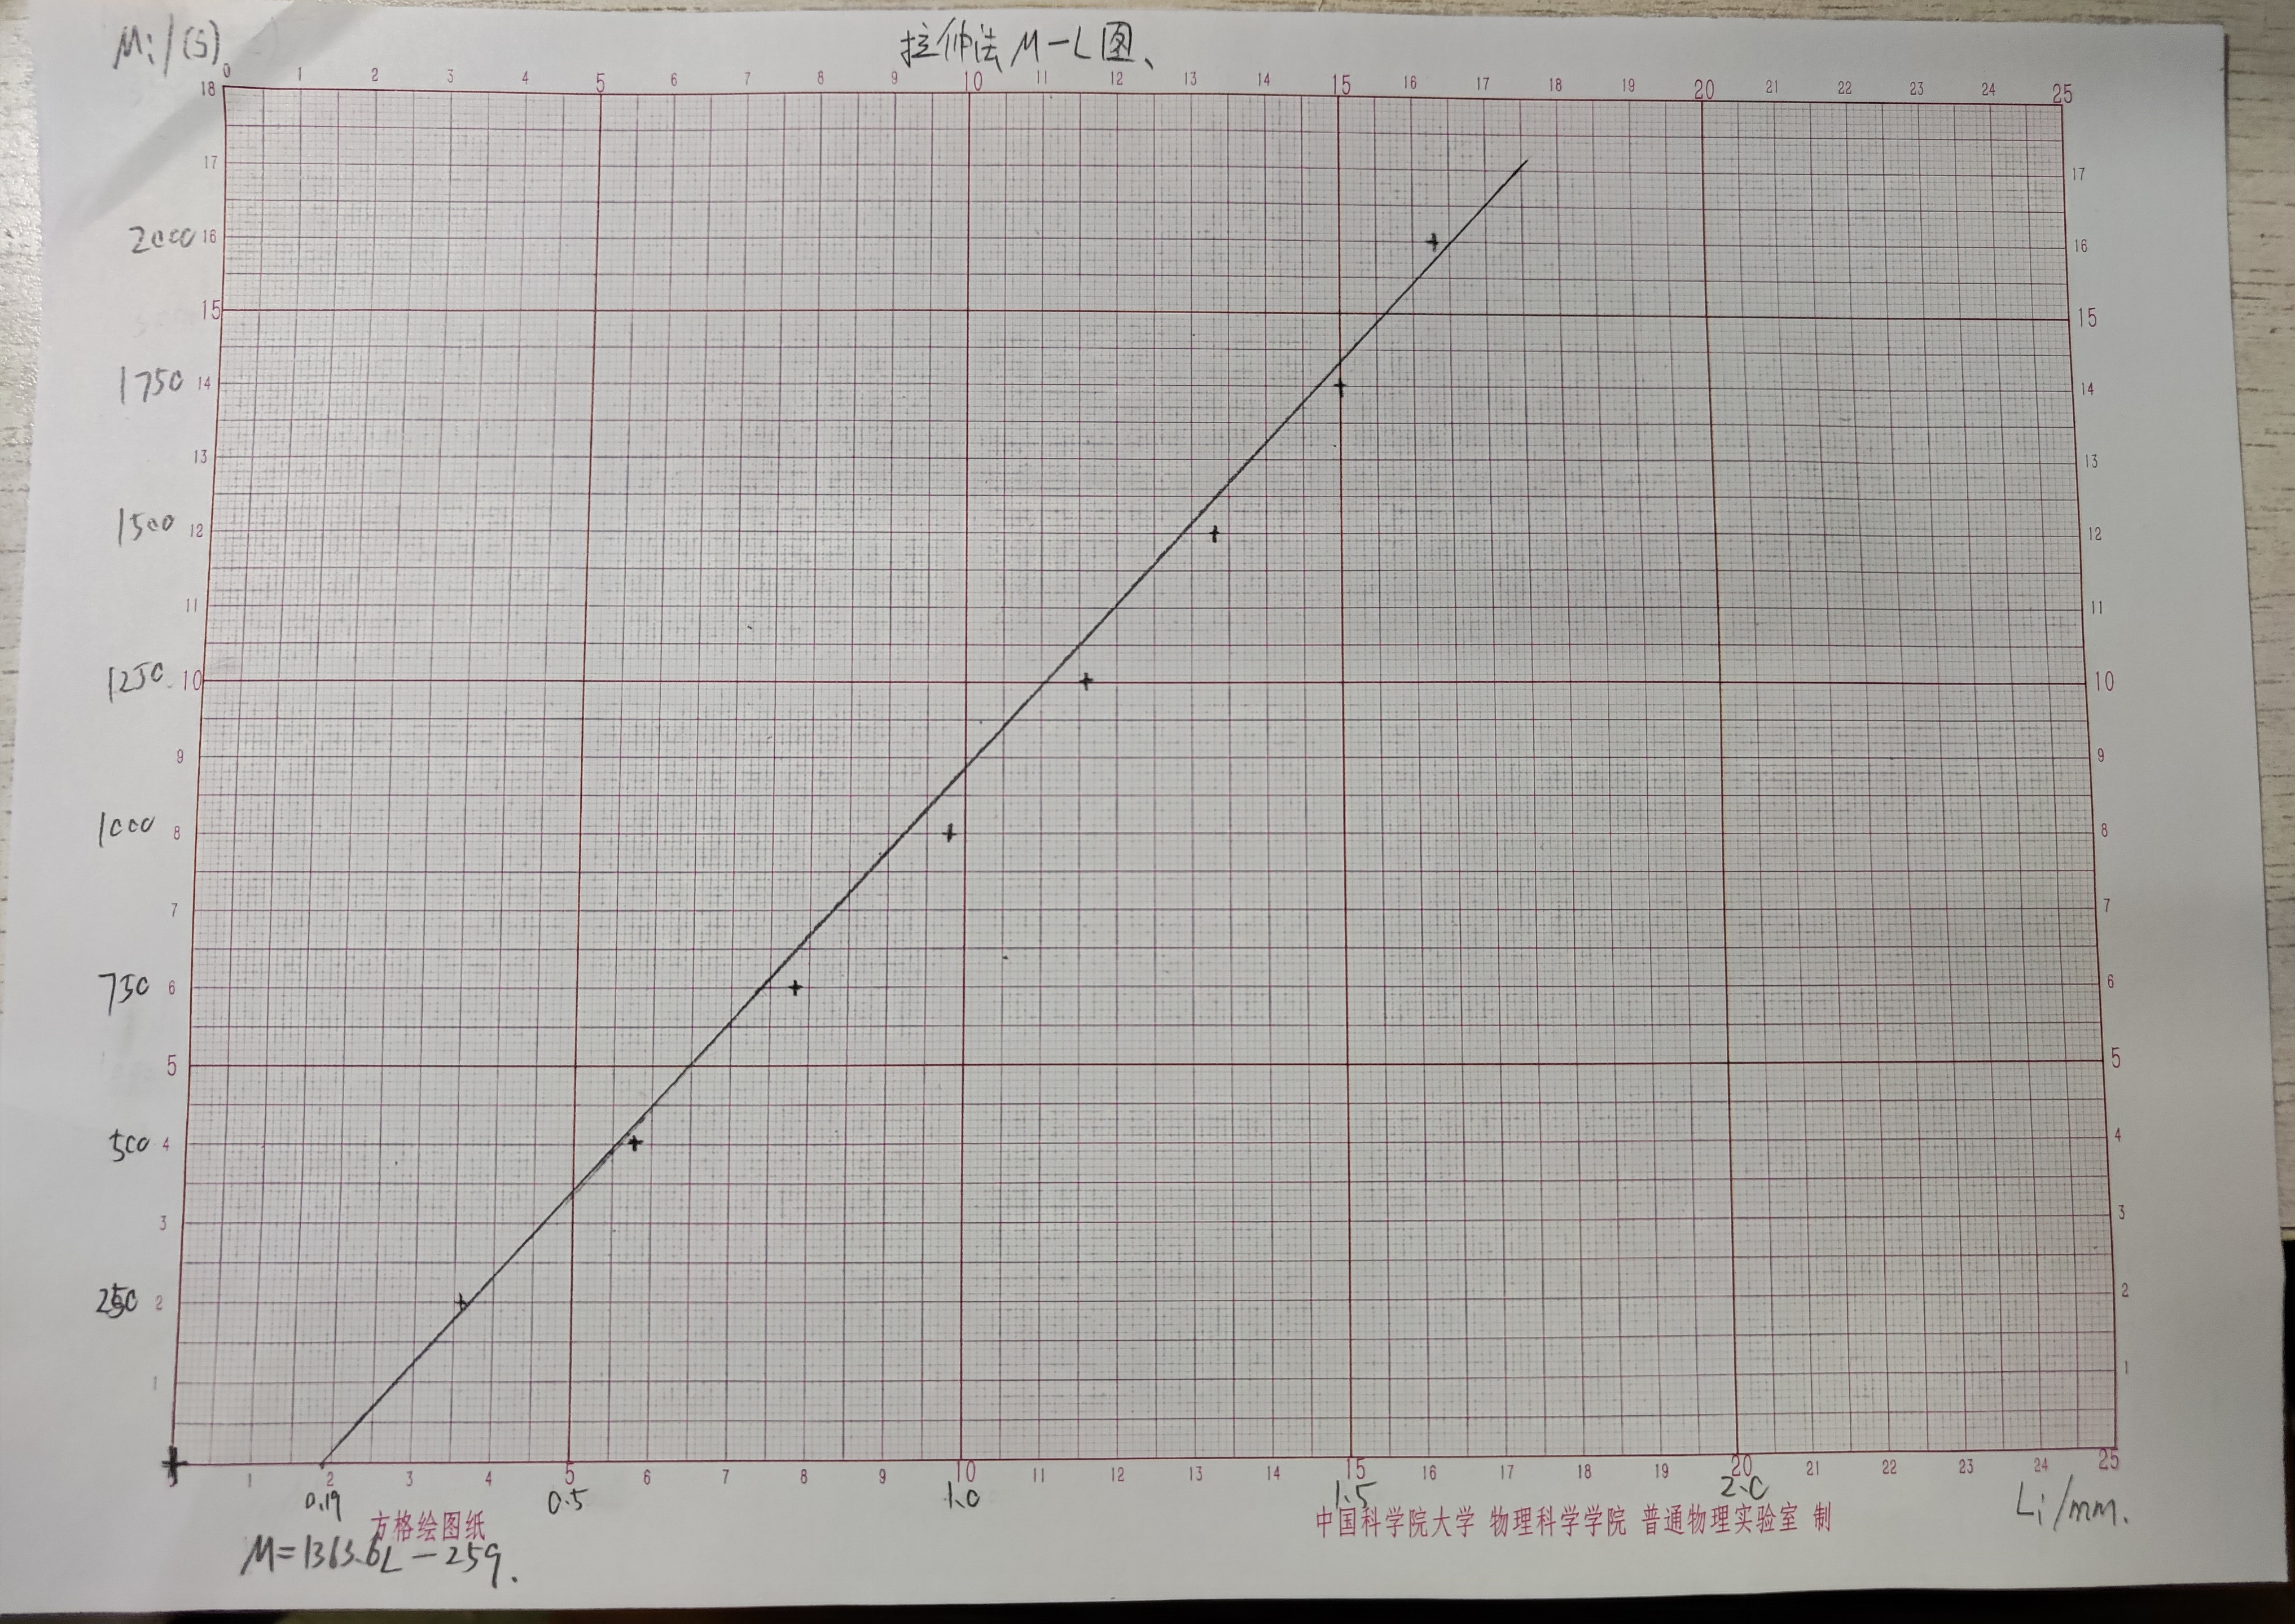
\includegraphics[width=7.5cm]{Fig/3.jpg}
        \caption{拉伸法M-L图(手画)}
        \label{fig:3}
    \end{minipage}
    \begin{minipage}[t]{0.49\linewidth}
        \centering
        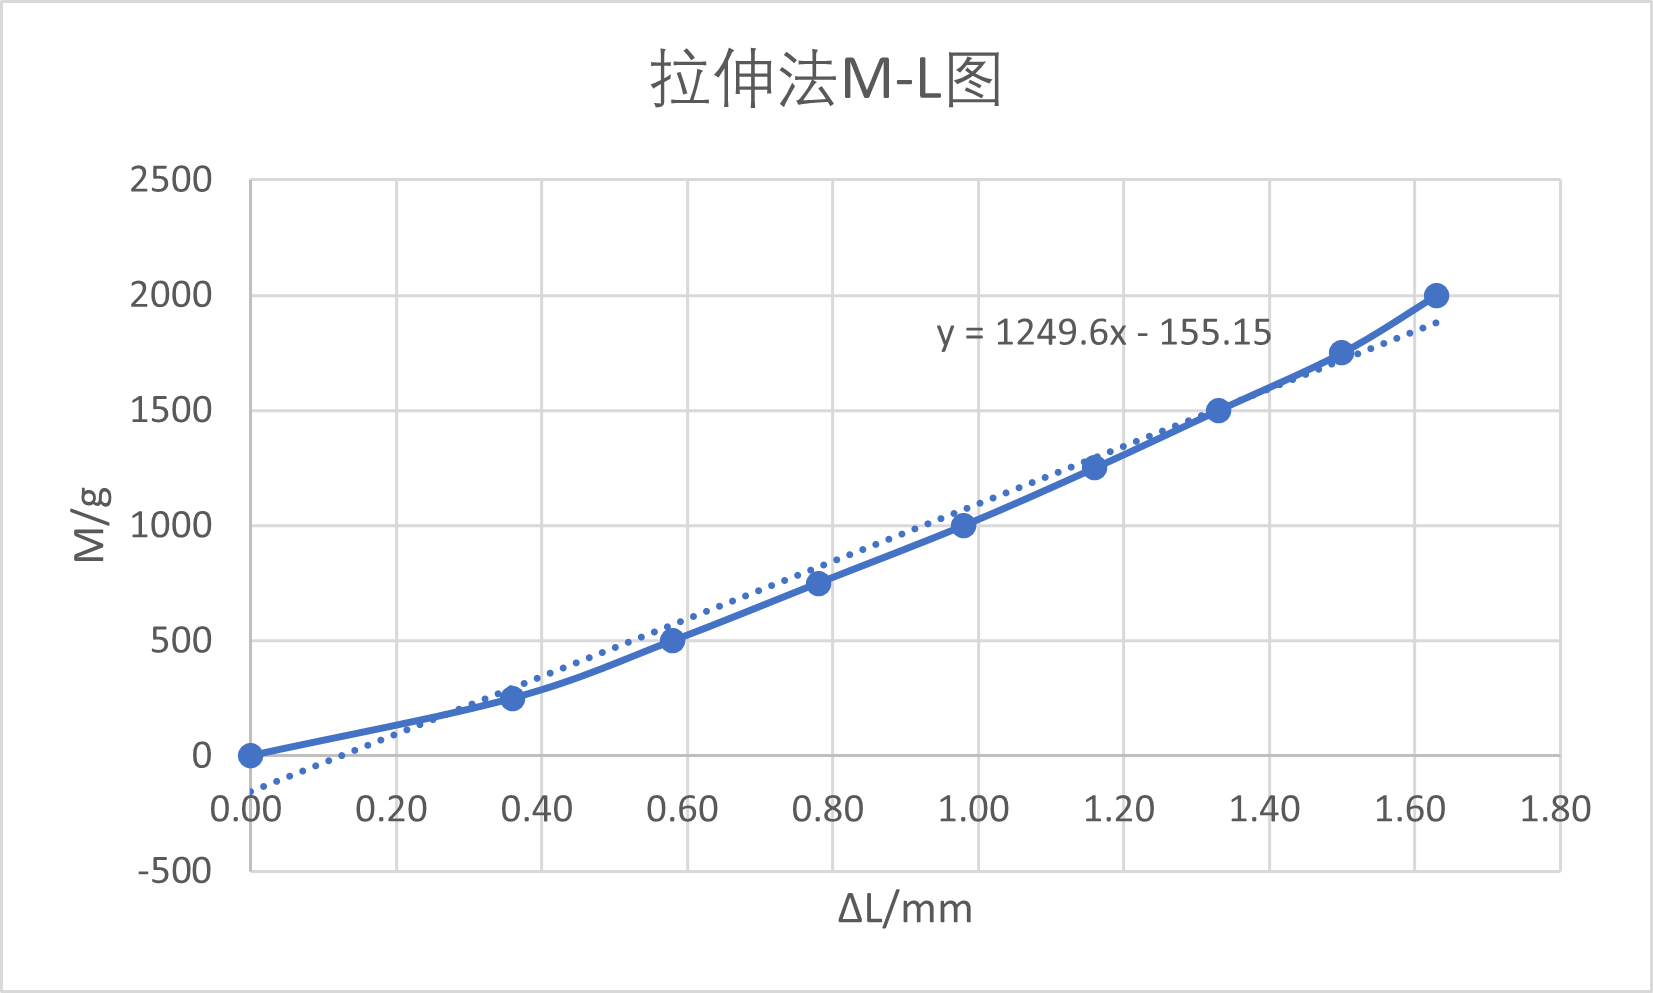
\includegraphics[width=7.5cm]{Fig/4.png}
        \caption{拉伸法M-L图(机画)}
        \label{fig:4}
    \end{minipage}
\end{figure}

\par \noindent 误差分析与不确定度:
\begin{enumerate}
    \item 长度L:
    \\ 3m钢卷尺分度值1mm,允差$\pm 2mm$。认为$u_{B1}$为分度值
    \[u_{B1}(L)=1.00mm\quad u_{B2}(L)=\frac{ 2mm}{\sqrt{3}}=1.15mm\quad u(L)=\sqrt{u_{B1}^2+u_{B2}^2}=1.52mm\]
    \item 直径d:
    \\25mm螺旋测微器分度值$0.01mm$,允差$\pm 0.005mm$。
    \[u_A(\bar{d})=\sqrt{\frac{\sum d_i-\bar{d}}{n(n-1)}}=0.0173mm\quad u_{B2}(\bar{d})=\frac{ 0.005mm}{\sqrt{3}}=0.0029mm\quad u(\bar{d})=\sqrt{u_A^2+u_{B2}^2}=0.0175mm\]
    \item 质量M:
    \\ 认为砝码质量的不确定度为千分之一,即$u(M)=0.25g$
    \item 伸长量l:
    \\ 显微镜量程4mm,分度值0.05mm,允差$\pm 0.005mm$。在测量加载和卸载长度时,进行两次测量取平均,认为$u_{B1}$为分度值的一半。
    \[u_{B1}(l)=0.025mm \quad u_{B2}(l)=\frac{ 0.005mm}{\sqrt{3}}=0.0029mm \quad u(l)=\sqrt{u_{B1}^2+u_{B2}^2}=0.025mm\]
    \item 由$Y=\frac{4MgL}{\pi d^2\Delta L}$
    \[{\left(\frac{u(Y)}{Y}\right)}^2={\left(\frac{u(M)}{M}\right)}^2+{\left(\frac{u(L)}{L}\right)}^2+{\left(2\frac{u(d)}{d}\right)}^2+{\left(\frac{u(l)}{l}\right)}^2\]
    计算得$u(Y)=20GPa$(取$Y=141GPa$)。误差率14\%。
\end{enumerate}



\subsection{使用霍尔传感器测杨氏模量(弯曲法)}
\noindent 实验步骤:
\begin{enumerate}
    \item 选择样品:(黄铜\makebox[3em][c]{\others},铸铁\makebox[3em][c]{\othersYes})。
    \item 用直尺测量两刀口间距d,用游标卡尺测量样品宽度b,用螺旋测微器测量样品厚度a,测量6次取平均值。
    \item 将样品安装在测定仪上。调整加力调节旋钮,使拉力绳拉紧。调整测量仪调零旋钮,使初始电压$i_0$和拉力绳上初始等效质量$M_0$近乎于0,并记录。
    \item 调整显微镜位置,使其能够良好读数。读取并记录显微镜初始读数,记为$Z_0$。
    \item 单向调整加力调节旋钮,每次增大10g,读取测量仪上示数,记录电压$U_i$和拉力绳上等效质量$M_i$。重复8次。
    \item 处理数据。将测量值$M_i,Z_i,U_i$修正为和初始值$M_0,Z_0,U_0$的差。计算$\Delta Z_i=Z_{i+4}-Z_i,\Delta U_i=U_{i+4}-U_i$,由逐差法,
    \[\Delta \bar{Z}=\frac{\sum_{i = 1}^{n} \Delta \bar{Z}_i }{n^2} \quad \Delta \bar{U}=\frac{\sum_{i = 1}^{n} \Delta \bar{U}_i }{n^2}\]
    计算$U_I^2,Z_i^2,Z_i \cdot U_i$。对上述数据取平均。
    \item 用作图法和最小二乘法处理数据。
\end{enumerate}
\noindent 实验数据:
\begin{table}[H]
    \centering
    \caption{霍尔法横梁几何尺寸}
    \begin{tabular}{|c|c|c|c|c|c|c|c|}
    \hline
        测量次数 & 1 & 2 & 3 & 4 & 5 & 6 & 平均值 \\ \hline
        长度$d/mm$ & 228.5  & 227.5  & 228.0  & 229.0  & 228.0  & 228.5  & 228.2  \\ \hline
        宽度$b/mm$ & 23.00  & 23.24  & 23.16  & 23.10  & 23.04  & 23.02  & 23.09  \\ \hline
        厚度$a/mm$ & 0.971  & 0.972  & 0.970  & 0.976  & 0.968  & 0.972  & 0.972 \\ \hline
    \end{tabular}
\end{table}
\par \hspace*{2em} 显微镜初始读数$Z_0=1.89mm$,电压初始读数$U_0=1mV$
\begin{table}[H]
    \centering
    \caption{霍尔法测量数据}
    \begin{tabular}{|c|c|c|c|c|c|c|c|c|}
    \hline
        $M_i/g$ & 0.6  & 10.0  & 20.9  & 30.5  & 40.1  & 50.3  & 60.1  & 69.9  \\ \hline
        $Z_i/mm$ & 1.89  & 1.97  & 2.09  & 2.16  & 2.22  & 2.29  & 2.35  & 2.41  \\ \hline
        $Z_{i\text{修正}}/mm$ & 0.00  & 0.08  & 0.20  & 0.27  & 0.33  & 0.40  & 0.46  & 0.52  \\ \hline
        $U_i/mV$ & 1 & 17 & 37 & 55 & 73 & 92 & 110 & 128 \\ \hline
        $U_{i\text{修正}}/mV$ & 0 & 16 & 36 & 54 & 72 & 91 & 109 & 127 \\ \hline
        $\Delta Z_i/mm$& 0.33 & 0.32 & 0.26 & 0.25 & ~ & ~ & ~ & ~ \\ \hline
        $\Delta U_i/mV$  & 72 & 75 & 73 & 73 & ~ & ~ & ~ & ~ \\ \hline
        $U_i^2/mV^2$ & 0 & 256 & 1296 & 2916 & 5184 & 8281 & 11881 & 16129 \\ \hline
        $Zi^2/mm^2$ & 0.00  & 0.01  & 0.04  & 0.07  & 0.11  & 0.16  & 0.21  & 0.27  \\ \hline
        $Z_iU_i/(mm\cdot mV)$ & 0.0  & 1.3  & 7.2  & 14.6  & 23.8  & 36.4  & 50.1  & 66.0 \\ \hline
    \end{tabular}
\end{table}
\begin{table}[H]
    \centering
    \begin{tabular}{|c|c|c|c|c|c|c|c|}
    \hline
        $\Delta Z_i/mm$ & $\Delta U_i/mV$ & $\sum Z_i$ & $\bar{Z_i}$  & $\sum U_i$ & $\bar{U_i}$  & $\sum Z_i^2$ & $\sum Z_i U_i$ \\ \hline
        0.0725 & 18.3 & 2.26 & 0.282 & 505 & 63.1 & 0.87 & 199 \\ \hline
    \end{tabular}
\end{table}
\begin{figure}[H]
    \centering
    \begin{minipage}[t]{0.49\linewidth}
        \centering
        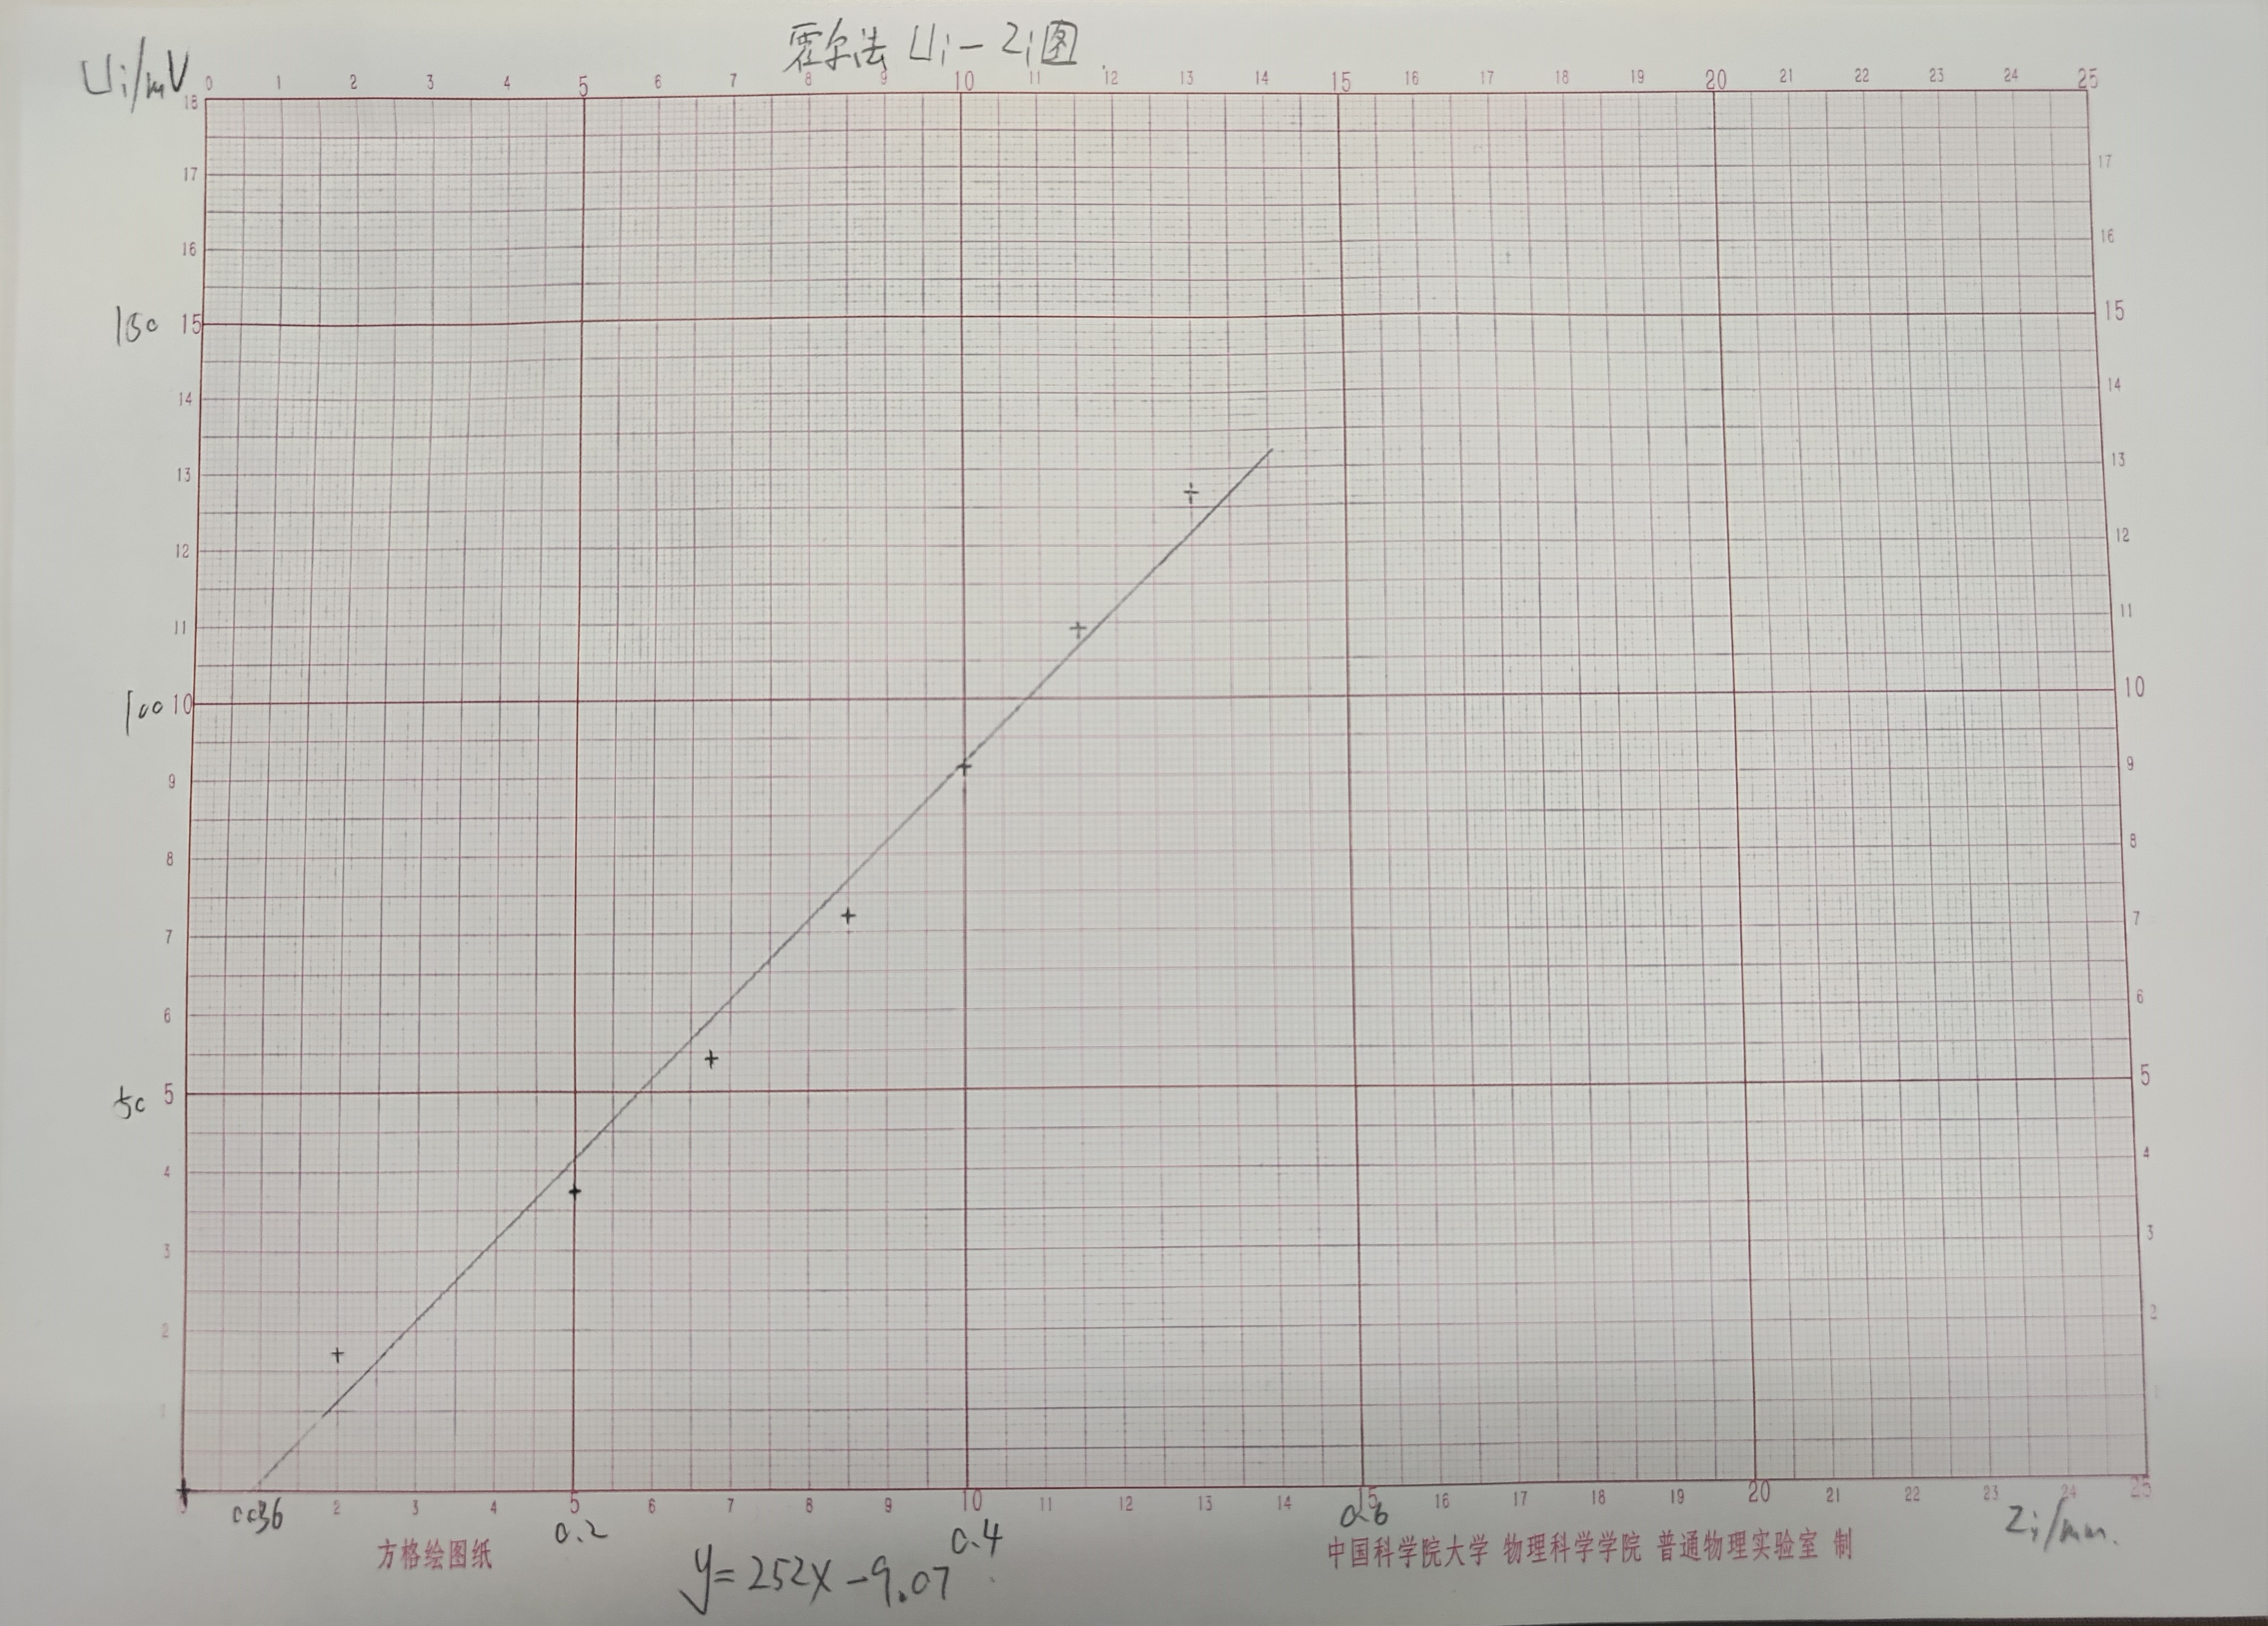
\includegraphics[width=7.5cm]{Fig/5.jpg}
        \caption{霍尔法U-Z图(手画)}
        \label{fig:5}
    \end{minipage}
    \begin{minipage}[t]{0.49\linewidth}
        \centering
        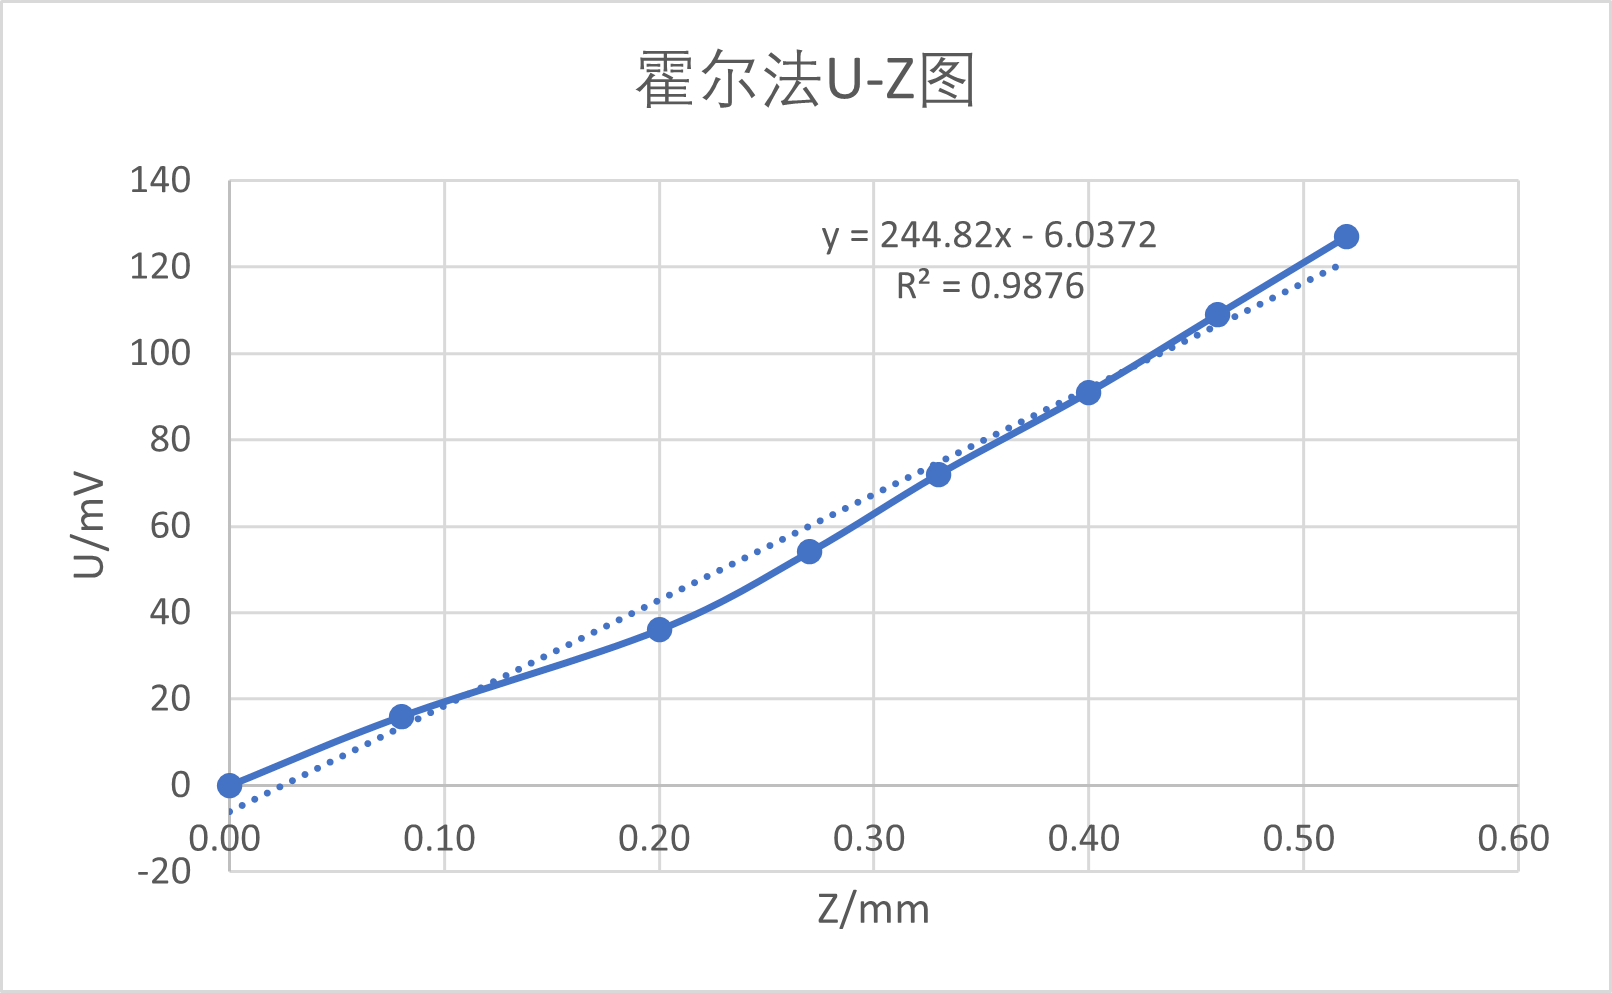
\includegraphics[width=7.5cm]{Fig/6.png}
        \caption{霍尔法U-Z图(机画)}
        \label{fig:6}
    \end{minipage}
\end{figure}
\par 由$E=\frac{d^3\cdot M g}{4a^3\cdot b\cdot\Delta Z}$,计算得$E=189GPa$
\par 由逐差法,$\frac{\Delta U_i}{\Delta Z_i}=252(mV\cdot {mm}^{-1})$
\par 由作图法,$k=\frac{\Delta U_i}{\Delta Z_i}=252 (mV\cdot {mm}^{-1}),b=-9.07(mV)$
\par 由最小二乘法,$k=243(mV\cdot {mm}^{-1}),b=-5.43(mV)$
\par 杨氏模量典型值$E=181.5GPa$,霍尔传感器灵敏度典型值$\frac{\Delta U_i}{\Delta Z_i}=250(mV\cdot {mm}^{-1})$。

\vspace*{1em}
\par \noindent 误差分析与不确定度:
\begin{enumerate}
    \item 长度d:由于直尺一段难以固定,估读位不确定,仅以0.05mm估读。
    \\ 30cm钢直尺分度值$0.1mm$,允差$\pm 0.12mm$。
    \[u_A(\bar{d})=\sqrt{\frac{\sum d_i-\bar{d}}{n(n-1)}}=0.289mm \quad u_{B2}(\bar{d})=\frac{0.12mm}{\sqrt{3}}=0.069mm\quad u(\bar{d})=\sqrt{u_A^2+u_{B2}^2}=0.297mm\]
    \item 宽度b:
    \\ 30cm游标卡尺分度值$0.02mm$,允差$\pm 0.04mm$。
    \[u_A(\bar{b})=\sqrt{\frac{\sum b_i-\bar{b}}{n(n-1)}}=0.121mm\quad u_{B2}(\bar{d})=\frac{0.04mm}{\sqrt{3}}=0.023mm\quad u(\bar{b})=\sqrt{u_A^2+u_{B2}^2}=0.123mm\]
    \item 厚度a:
    \\ 25mm螺旋测微器分度值$0.01mm$,允差$\pm 0.004mm$。
    \[u_A(\bar{a})=\sqrt{\frac{\sum a_i-\bar{a}}{n(n-1)}}=0.0191mm\quad u_{B2}(\bar{a})=\frac{ 0.004mm}{\sqrt{3}}=0.0023mm\quad u(\bar{a})=\sqrt{u_A^2+u_{B2}^2}=0.0192mm\]
    \item 电压U:
    \\ 量程1:0-199.9mV,分度值0.1mV。认为不确定度为分度值,$u(U)=0.1mV$
    \item 位移Z:
    \\ 显微镜量程0-6mm,目镜测微鼓轮最小分度值0.01mm,鼓轮实际读数最小分辨率0.01/2=0.005mm。认为不确定度为鼓轮实际读数最小分辨率,$u(Z)=0.005mm$。
    \item 质量M:
    \\ 量程0-199.9g,分度值0.1g。认为不确定度为分度值,$u(M)=0.1g$
    \item 杨氏模量E:
    \item 由$E=\frac{d^3\cdot M g}{4a^3\cdot b\cdot\Delta Z}$
    \[{\left(\frac{u(E)}{E}\right)}^2={\left(3\frac{u(d)}{d}\right)}^2+{\left(\frac{u(M)}{M}\right)}^2+{\left(3\frac{u(a)}{a}\right)}^2+{\left(\frac{u(b)}{b}\right)}^2+{\left(\frac{u(Z)}{Z}\right)}^2\]
    $u(E)=20GPa$,于是测量值杨氏模量$E=189GPa \pm 20GPa$,给定参考值属于此区间,说明实验测量良好。误差率10\%。
\end{enumerate}


\subsection{动态悬挂法测杨氏模量}
\noindent 实验步骤:
\begin{enumerate}
    \item 选择样品:(黄铜\makebox[3em][c]{\others},铸铁\makebox[3em][c]{\othersYes})。
    \item 用游标卡尺测样品的长度L和直径d,用电子天秤测样品质量m,并记录。
    \item 打开仪器。调整悬挂点位置x。调整悬丝使样品保持水平。调整输入频率,使得在示波器上振幅最大,记录共振频率$f_1$。依照表格进行8组实验。
    \item 处理数据。计算$\frac{x}{L}$。
    \item 用作图法和最小二乘法处理数据。
\end{enumerate}
\noindent 实验数据:
\par 样品:铝\qquad 长度$L=179.84mm$\qquad 直径$d=6.04mm$ \qquad 样品质量$m=13.62g$
\begin{figure}[H]
    \centering
    \begin{minipage}[t]{0.49\linewidth}
        \centering
        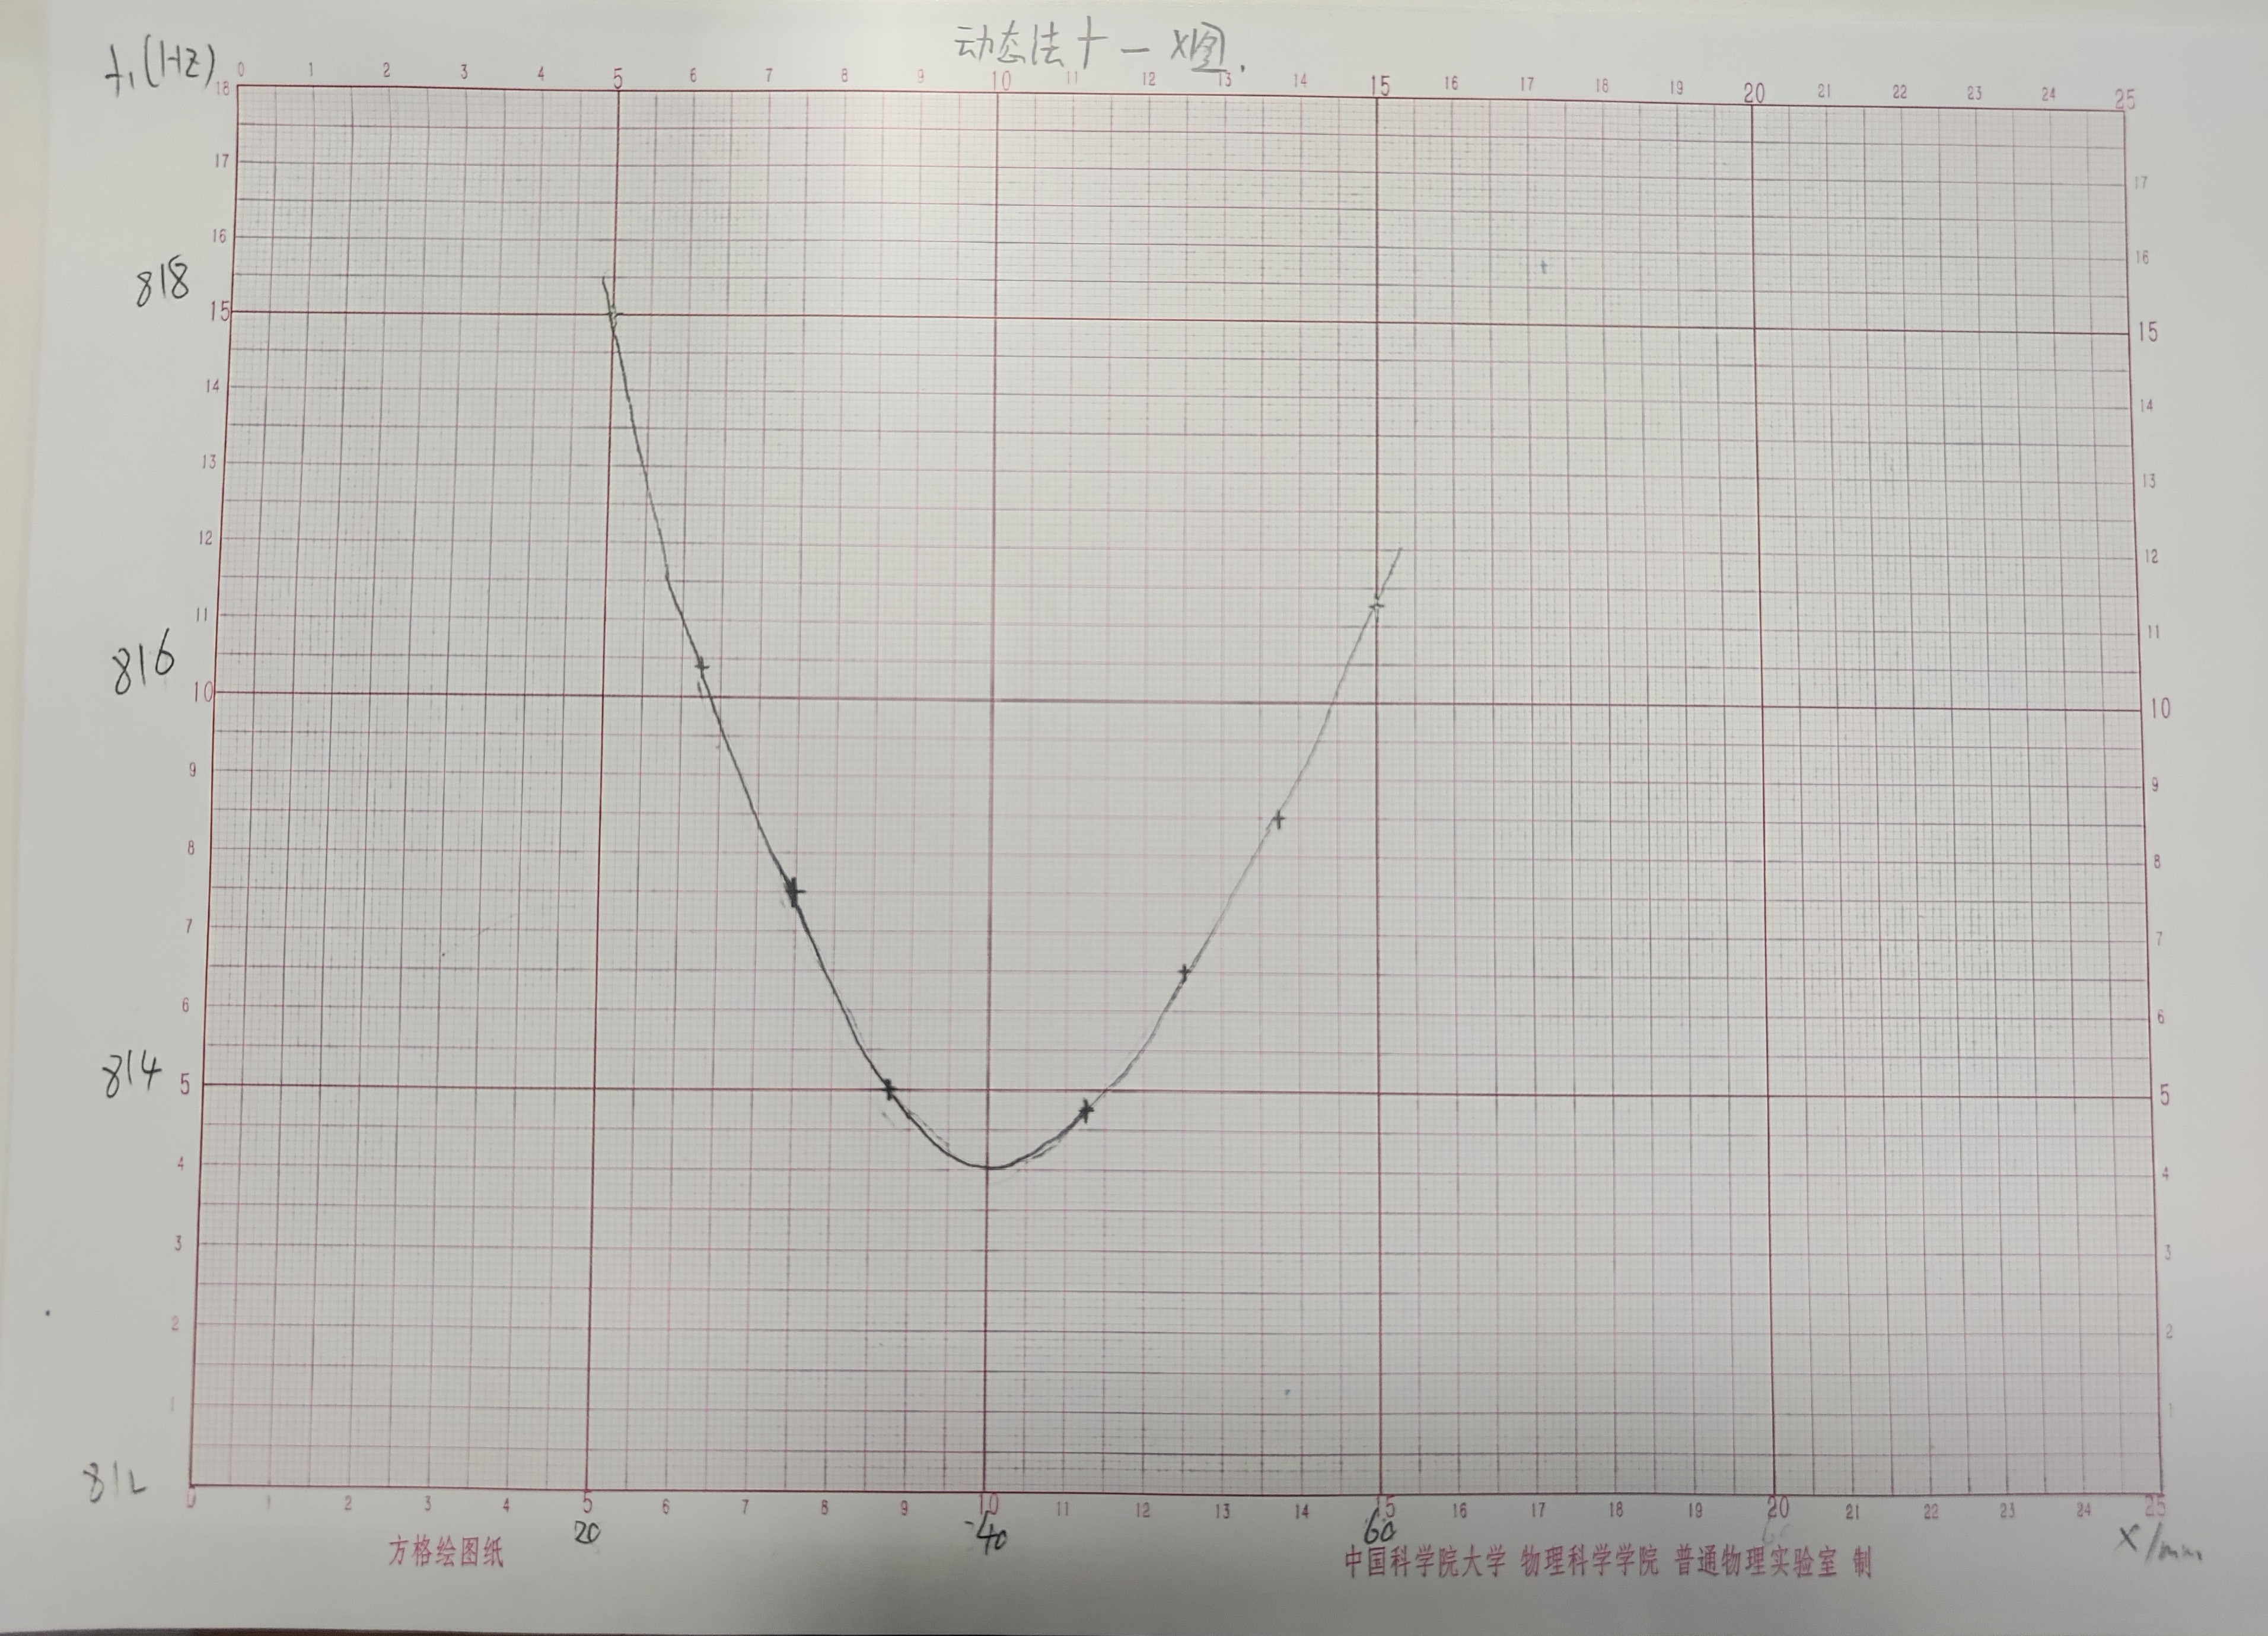
\includegraphics[width=7.5cm]{Fig/7.jpg}
        \caption{动态法f-x图(手画)}
        \label{fig:7}
    \end{minipage}
    \begin{minipage}[t]{0.49\linewidth}
        \centering
        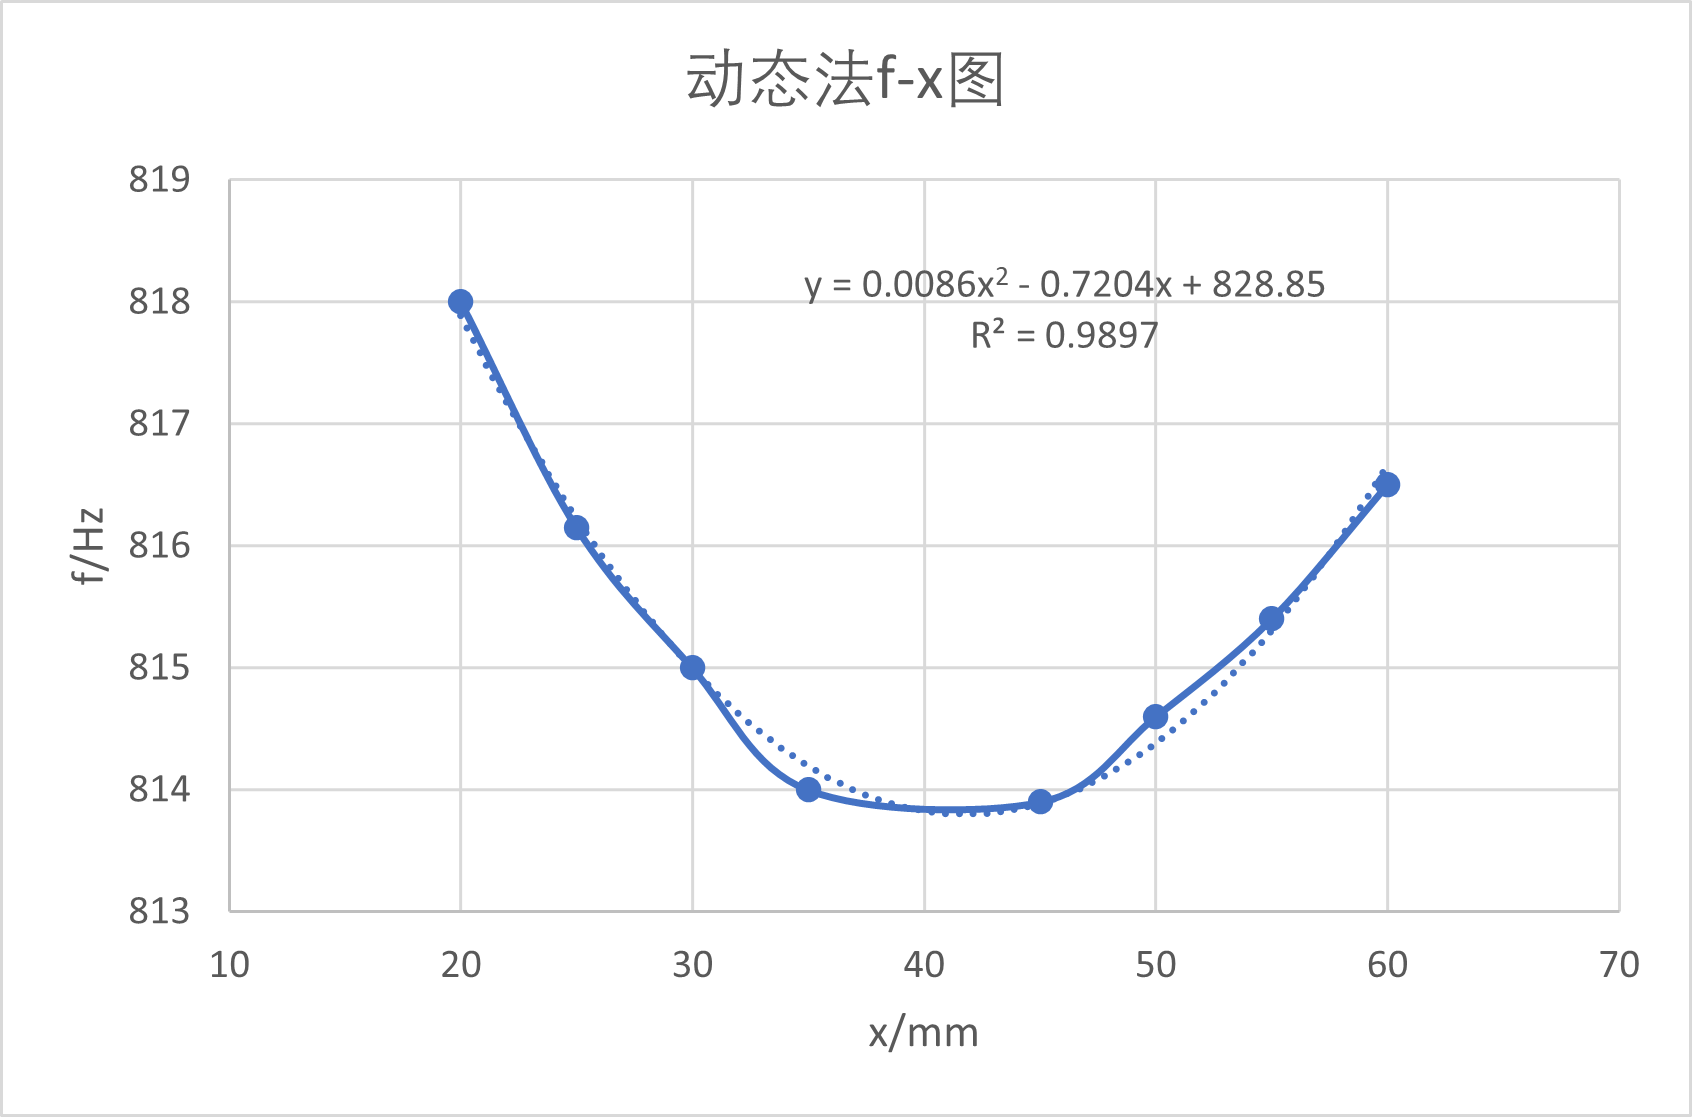
\includegraphics[width=7.5cm]{Fig/8.png}
        \caption{动态法f-x图(机画)}
        \label{fig:8}
    \end{minipage}
\end{figure}
\par 作图法得最小值$f_1=813.6Hz$。杨氏模量$Y=1.6067\frac{L^3mf_1^2}{d^4}=63.3GPa$
\par 电脑作图得最小值$f_1=813.76Hz$。$Y=1.6067\frac{L^3mf_1^2}{d^4}=63.3GPa$
\par 最小二乘法:设$y=Ax^2+Bx+C$,由线性方程组
\begin{equation}
    \begin{cases}
        \left(\sum\limits_{i=1}^{n}x_i^4\right)A+\left(\sum\limits_{i=1}^{n} x_i^3\right)B+\left(\sum\limits_{i=1}^{n} x_i^2\right)C= \left(\sum\limits_{i=1}^{n} y_i x_i^2\right) \\
        \left(\sum\limits_{i=1}^{n} x_i^3\right)A+\left(\sum\limits_{i=1}^{n} x_i^2\right)B+\left(\sum\limits_{i=1}^{n} x_i\right)C= \left(\sum\limits_{i=1}^{n} y_i x_i\right) \\
        \left(\sum\limits_{i=1}^{n} x_i^2\right)A+\left(\sum\limits_{i=1}^{n} x_i\right)B+nC= \left(\sum\limits_{i=1}^{n} y_i\right) \\
    \end{cases}
\end{equation}
可解出A,B,C。解得
\begin{equation}
    C=\frac{b_5a_6-b_4a_7}{a_6a_8-a_7^2}
    \qquad B=\frac{b_4-a_7C}{a_6}
    \qquad A=\frac{b_1-a_2B-a_3C}{a_1}
\end{equation}
其中
\[a_1=\sum x_i^4 \quad a_2=\sum x_i^3 \quad a_3=\sum x_i^2 \quad a_4=\sum  x_i \quad a_5=n \quad a_6=a_1a_3-a_2^2 \quad a_7=a_1a_4-a_2a_3 \quad a_8=a_1a_5-a_3^2\]
\[b_1=\sum y_i x_i^2 \quad b_2=\sum y_i x_i \quad b_3=\sum y_i \quad b_4=b_2a_1-b_1a_2 \quad b_5=b_3a_1-b_1a_3\]
\begin{table}[H]
    \centering
    \begin{tabular}{|c|c|c|c|c|c|c|c|}
    \hline
        a1 & a2 & a3 & a4 & a5 & a6 & a7 & a8 \\ \hline
        3.532E7 & 6.92E5 & 1.43E4 & 3.2E2 & 8 & 2.625E10 & 1.408E9 & 7.809E7 \\ \hline
        b1 & b2 & b3 & b4 & b5 & ~ & ~ & ~ \\ \hline
        1.166E7 & 2.609E5 & 6.524E3 & 1.148E12 & 6.371E10 & ~ & ~ & ~\\ \hline
    \end{tabular}
\end{table}
解得\[C=830.93\qquad B=-0.8362 \qquad A=0.01008\]%41.48
最小值$f_1=813.59Hz$,杨氏模量$Y=1.6067\frac{L^3mf_1^2}{d^4}=63.3GPa$
\par 本实验使用的铝条,铝的杨氏模量典型值$Y=70GPa$。

\par \noindent 误差分析与不确定度:
\begin{enumerate}
    \item 长度L:
    \\ 30cm游标卡尺分度值$0.02mm$,允差$\pm 0.04mm$。认为$u_{B1}$为分度值。
    \[u_{B1}(L)=0.02mm\quad u_{B2}(L)=\frac{0.04mm}{\sqrt{3}}=0.023mm\quad u(L)=\sqrt{u_{B1}^2+u_{B2}^2}=0.030mm\]
    \item 直径d:
    \\ 25mm螺旋测微器分度值$0.01mm$,允差$\pm 0.004mm$。认为$u_{B1}$为分度值的一半。
    \[u_{B_1}(d)=0.005mm\quad u_{B2}(d)=\frac{ 0.004mm}{\sqrt{3}}=0.0023mm\quad u(d)=\sqrt{u_A^2+u_{B2}^2}=0.0055mm\]
    \item 质量m:
    \\ 电子天平分度值0.01g,认为$u(m)=0.01g$为分度值。
    \item 振动频率f:
    \\ 最小分度值0.001Hz。本实验中,每次调整0.1Hz,若调整过小难以区分示波器上图像差别。认为不确定度为调整量,$u(f)=0.1Hz$。
    \item 由$Y=1.6067\frac{L^3mf_1^2}{d^4}$
    \[{\left(\frac{u(Y)}{Y}\right)}^2={\left(3\frac{u(L)}{L}\right)}^2+{\left(\frac{u(m)}{m}\right)}^2+{\left(2\frac{u(f_1)}{f_1}\right)}^2+{\left(4\frac{u(d)}{d}\right)}^2\]
    计算得$u(Y)=0.2GPa$(取$Y=63.3GPa$)。误差率0.3\%。则测量值$Y=63.3GPa \pm 0.2GPa$。
\end{enumerate}



\section{实验反思、收获与总结}
\subsection{拉伸法思考题}
\begin{enumerate}
    \item 杨氏模量测量数据N 若不用逐差法而用作图法,如何处理?
    \par \hspace*{2em}斜率$k\frac{\pi d^2 }{4gL}Y$,作图法得到直线斜率后即可得到杨氏模量。
    \item 两根材料相同但粗细不同的金属丝,它们的杨氏模量相同吗?为什么?
    \par \hspace*{2em} 在粗细相差不大时,金属丝在拉伸过程中直径变化可忽略,因此杨氏模量相同。杨氏模量公式中含有$d^2$项,直径的改变被考虑在测量中。 
    \item 本实验使用了哪些测量长度的量具?选择它们的依据是什么?它们的仪器误差各是多少?
    \par \hspace*{2em}用钢卷尺测钼丝长度,用螺旋测微器测钼丝直径,用CCD测伸长量。
    \par \hspace*{2em}卷尺量程大。螺旋测微器精度高但量程小,专用于夹取物品的测量。CCD实质为微小直尺,量程小但精度高。
    \par \hspace*{2em}卷尺量程3m,分度值1mm,允差$\pm 2mm$。螺旋测微器量程25mm,分度值$0.01mm$,允差$\pm 0.005mm$。显微镜量程4mm,分度值0.05mm,允差$\pm 0.005mm$。
    \item 在CCD 法测定金属丝杨氏模量实验中,为什么起始时要加一定数量的底码?
    \par \hspace*{2em}不加外力时,金属丝可能未处于拉直状态。我实验时忘记加底码了。在电脑作图中,可以看到前两个点较为异常,加底码后可使其不影响后续数据。
    \item 加砝码后标示横线在屏幕上可能上下颤动不停,不能够完全稳定时,如何判定正确读数?
    \par \hspace*{2em}首先轻轻碰一下砝码处让其颤动减弱,之后就能良好读数。
    \item 金属丝存在折弯使测量结果如何变化?
    \par \hspace*{2em}弯折的金属丝相当于弹簧,弹簧的弹性系数远小于杨氏模量,因此会给杨氏模量测量带来巨大误差。事实上,我们使用的仪器金属丝有多个弯折。在依次加砝码时,有些弯折可能被部分拉直,但这部分长度变化不是金属杨氏模量的贡献。而加载和卸载测两次长度取平均,能够降低此误差。
    \item 用螺旋测微器或游标卡尺测量时,如果初始状态都不在零位因此需要读出值减初值,对测量值的误差有何影响?
    \par \hspace*{2em}会增大仪器允差。本实验中测量仪器良好,初始状态都在零位,不用考虑。
\end{enumerate}
\subsection{霍尔法思考题}
\begin{enumerate}
    \item 弯曲法测杨氏模量实验,主要测量误差有哪些?请估算各因素的不确定度。
    \par \hspace*{2em}不确定度计算在上文。d为两刀口之间的距离,
    \[\left(\frac{u(d)}{d}\right)=0.13\% \qquad \left(\frac{u(M)}{M}\right)=1\% \qquad\left(\frac{u(a)}{a}\right)=2.0\% \qquad\left(\frac{u(b)}{b}\right)=0.53\% \qquad\left(\frac{u(Z)}{Z}\right)=6.9\%\]
    可以看到,伸长量Z为主要误差来源。叠加上次方项,厚度a的误差量也很大。
    \item 用霍尔位置传感器法测位移有什么优点?
    \par \hspace*{2em}由$\Delta U_H=K\cdot I \cdot \frac{dB}{dZ} \cdot\Delta Z$,在灵敏度K,电流I,磁场变化率$\frac{dB}{dZ}$相同的情况下,位移较小时保持线性。因此可以不用显微镜测量位移,而是用霍尔传感器测量电压,减小了位移测量的不确定度。
\end{enumerate}

\subsection{动态法思考题}
\begin{enumerate}
    \item 外延测量法有什么特点?使用时应注意什么问题?
    \par \hspace*{2em}外延法利用图像的延长,取得难以测量的量。本实验中波节上共振频率最小,但振幅几乎为0难以测量。实验外延法拟合图像即可得最小频率,也就是共振频率。使用时要注意测量点数量不能太少,且没有突变情况,否则拟合结果不准确。
    \item 物体的固有频率和共振频率有什么不同?它们之间有何关系?
    \par \hspace*{2em}在实验原理部分3.5已经叙述。
\end{enumerate}
\subsection{个人反思}
\begin{enumerate}
    \item 首先,实验时我忘记了千分尺要估读,因此进行了重测。
    \item 测量时,对于一些旋钮要单向调节,否则齿轮间隙差会造成误差。这个效应在霍尔法调节加力旋钮时特别明显。因此我在这部分测量进行了重测,第二次注意了这点。
    \item 本实验是我第一次用不确定度考虑误差,发现实验误差相当之大是有原因的。通过不确定度分析,能分析出哪个部分的误差较大,从而能够提出改进实验的方法。
    \item 在钼丝长度测量时,悬垂的钼丝难以测量准确长度,加上钢卷尺难以使用,这部分造成微小误差。
    \item 根据不确定度的原理,能够解释多次测量取平均,提高测量间隔,增大样品尺度都能够减小误差。
\end{enumerate}

\begin{center}
    \vspace*{1em}
    \Large \bf 第二部分\qquad 实验原始记录
\end{center}
\includepdf[pages={1-4}]{Data/杨氏模量实验数据.pdf}

\end{document}